\documentclass{article}
\usepackage{graphicx}
\usepackage[utf8]{vietnam}

\title{Labwork 3 Report}
\author{Pham Quang Duong - 2540048}
\date{}

\begin{document}

\maketitle

\section{Implementation \& Results}

For this assignment, we use An RGB image of size $4536 \times 8064$ to load and reshape it into $36,578,304 \times 3$ RGB values. Grayscale conversion was implemented using a CPU for-loop and a Numba CUDA kernel. The \texttt{time.time()} function was used to execute time measurement.

The CPU execution time was approximately 34.71 s and the GPU execution time was approximately 0.05 s, the execution time of GPU is faster than CPU $694.2\times$.

\section{Block Size Experiment}

We also ran a series of tests to see how tweaking the CUDA block size affects overall kernel execution. By adjusting the thread block size from 8 to 512, we see a clear trend in which the execution time drops noticeably at the start—falling from $0.075$ seconds to around $0.0491$ seconds. 

The sweet spot in our setup was a block size of 512, which recorded the fastest execution time at $0.0491$ seconds. Once the block size reached 64 and above, the performance gains flattened out and the execution times remained fairly steady.

\begin{center}
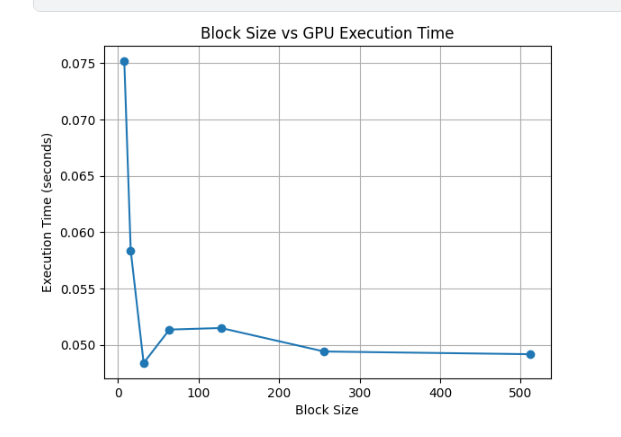
\includegraphics[width=0.8\textwidth]{blocksize.png}
\end{center}

\end{document}